\pagestyle{empty}
\cleardoublepage
\pagestyle{fancy}
\chapter{Evolução de Modularidade em Diferentes Regimes de
Seleção}\label{cap4}

\section{Introdução}

Neste capitulo vamos utilizar o modelo com matriz $B$ apresentado no
capítulo \ref{cap2} e parametrizado no capítulo \ref{cap3} para estudar
algumas possibilidades de trajetórias evolutivas responsáveis por moldar
populações na natureza. 
Novamente estamos interessados principalmente na evolução dos padrões de
covariação e surgimento de modularidade. 
Os parametros gerais usados nessas simulações são $p = 10$, $m = 50$
$\mu/\mu_B = 5$, $Ne = 5000$. 

\section{Estabelecimento de equilíbrio}

Afim de minimizar ao máximo a influência de estados iniciais das
populações, todas as simulações nesse capítulo são baseadas na mesma
população inicial, que por sua vez passou por 10000 gerações de deriva
pura, sem seleção de qualquer tipo, seguidos de 10000 gerações de
seleção estabilizadora correlacionada com matriz $\omega$ com dois
módulos, como na equação \ref{matw}. 
No primeiro periodo, de deriva, garantimos que o estado inicial é
totalmente perdido por ação de mutação e deriva. 
Depois, durante a seleção estabilizadora, garantimos que a população
esteja em equilibrio seleção-mutação-deriva, mas ainda com variação
suficiente para responder à seleção direcional. 
Padronizando as populações iniciais podemos isolar de forma mais
sistemática efeitos de diferentes regimes de seleção. 
Na figura \ref{varBurnin} observamos a evolução das variâncias
fenotípicas, variâncias genéticas dos valores aditivos e da
herdabilidade para todos os 10 traços da população. 
Notamos que incialmente as variâncias crescem rapidamente, pois sem
seleção a mutação introduz nova variação a cada geração que só pode ser
removida por deriva. 
Como a população é bastante grande ($Ne = 5000$), a remoção é lenta e o
equilibrio mutação-deriva se dá num valor de variância muito alto
(comparado com a variância ambiental ou variância do erro $e$, veja
capítulo \ref{cap2}, equação \ref{matrizB}). 
Nas mesmas figuras, após X gerações de deriva, foi imposto um regime de
seleção estabilizadora correlacionada. 
Imediatamente as variâncias genéticas e fenotípicas caem bruscamente
para os valores de equilibrio seleção-mutação-deriva, e o sistema se
estabiliza nesses valores. 
Podemos ver no painel \ref{Corr} o efeito sobre as correlações,
que também diminuem (?????). 

\begin{center}
   \begin{figure}[htbp]
      \centering
      \subfloat [Variâncias Fenotípicas]{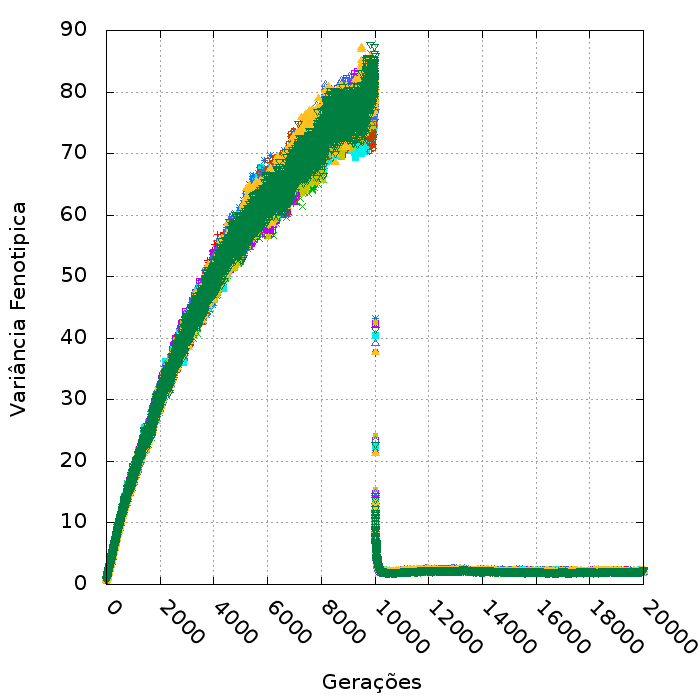
\includegraphics[width=70mm, height=70mm]{figuras/varBurninP.png}}\vspace{11pt}
      \subfloat [Variâncias Genéticas]{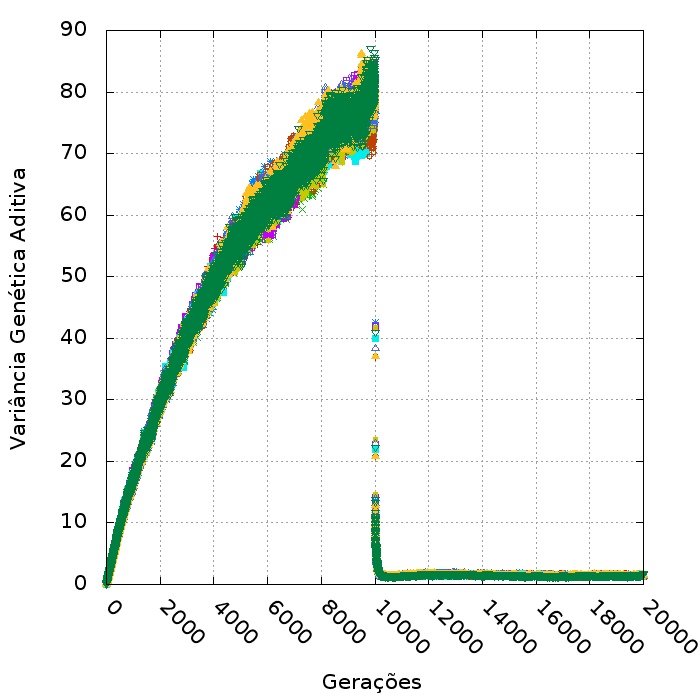
\includegraphics[width=70mm, height=70mm]{figuras/varBurninG.png}}\\ 
      \vspace{-18pt}
      \subfloat [Herdabilidade]{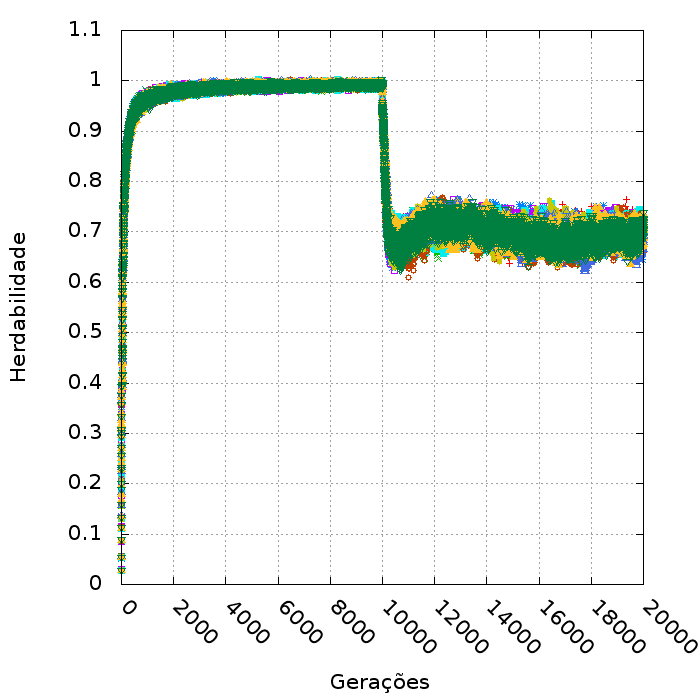
\includegraphics[width=70mm, height=70mm]{figuras/varBurninH.png}}\vspace{11pt} 
      \subfloat [Correlações]{\label{Corr}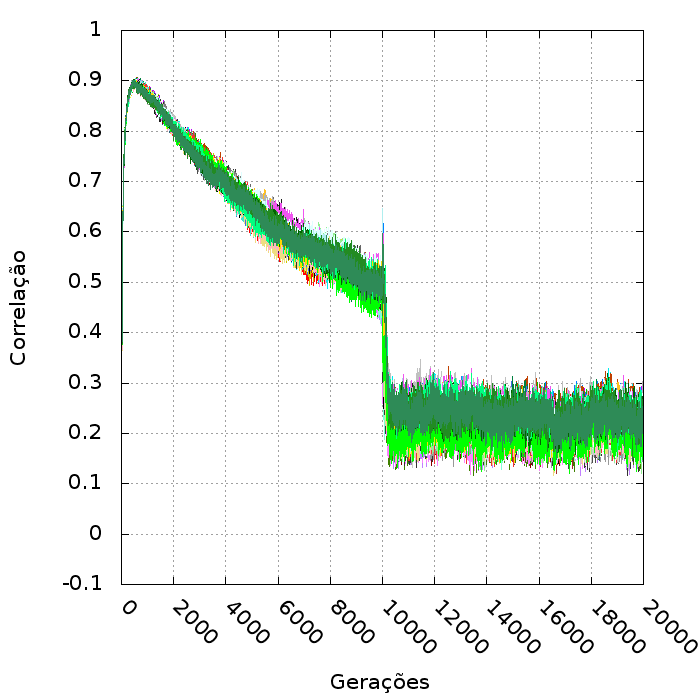
\includegraphics[width=70mm, height=70mm]{figuras/varBurninCorr.png}}\\
      \caption{População mandando brasa nas paradas}
      \label{varBurnin}
   \end{figure}
\end{center}

Tomados esses cuidados com a inicialização da população, iniciamos o
regime de seleção direcional com intensidade variaveis, como na seção
\ref{cap3:DirecB}. 
Novamente nossa seleção é medida por mudanças no pico adaptativo, com
$\Delta_S$ de $0.01$ até $0.2$. 
Valores de AVG-Ratio e modularidade $L$ para essas corridas podem ser
vistos nas figuras \ref{MFMStats1} e \ref{MFMStats2}. 
Incluimos também as últimas gerações de seleção estabilizadora por
clareza, a seleção direcional começa a atual a partir da geração 20000.  


\begin{center}
   \begin{figure}[htbp]
      \centering
      \subfloat [$\Delta_S = 0.01$]{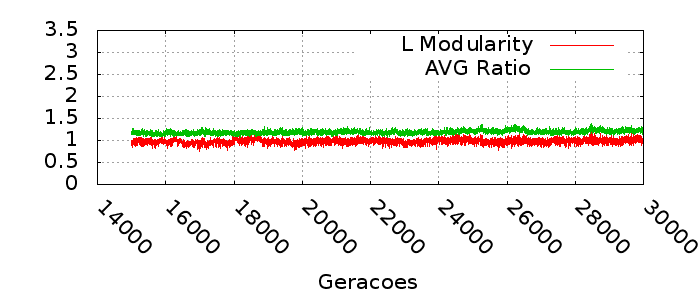
\includegraphics[width=70mm, height=30mm]{figuras/MFMStats10.png}}\vspace{11pt}
      \subfloat [$\Delta_S = 0.02$]{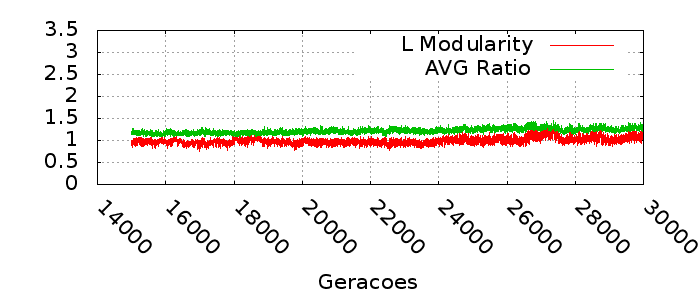
\includegraphics[width=70mm, height=30mm]{figuras/MFMStats20.png}}\\ 
      \vspace{-18pt}
      \subfloat [$\Delta_S = 0.03$]{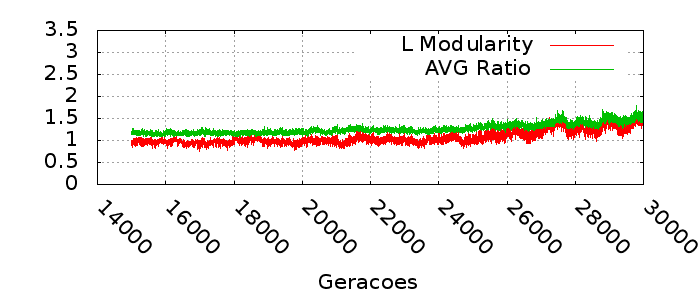
\includegraphics[width=70mm, height=30mm]{figuras/MFMStats30.png}}\vspace{11pt} 
      \subfloat [$\Delta_S = 0.04$]{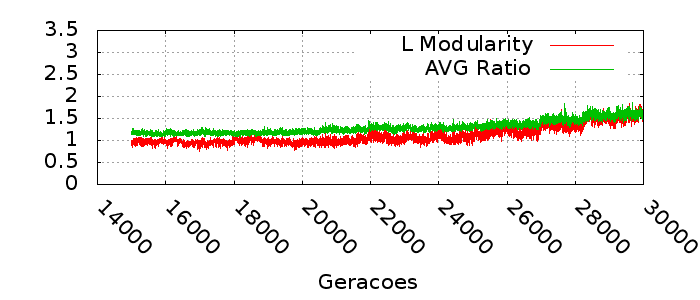
\includegraphics[width=70mm, height=30mm]{figuras/MFMStats40.png}}\\
      \vspace{-18pt}
      \subfloat [$\Delta_S = 0.05$]{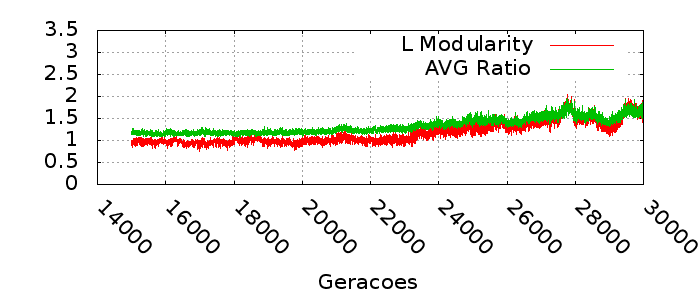
\includegraphics[width=70mm, height=30mm]{figuras/MFMStats50.png}}\vspace{11pt}
      \subfloat [$\Delta_S = 0.06$]{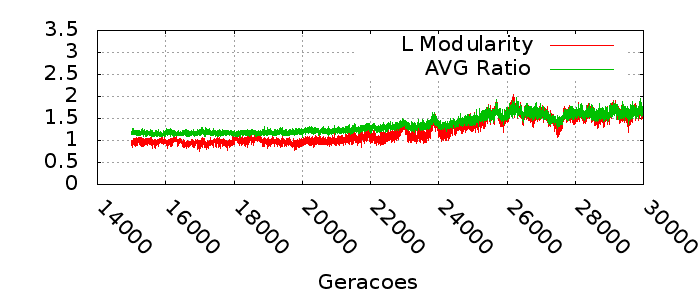
\includegraphics[width=70mm, height=30mm]{figuras/MFMStats60.png}}\\
      \vspace{-18pt}
      \subfloat [$\Delta_S = 0.07$]{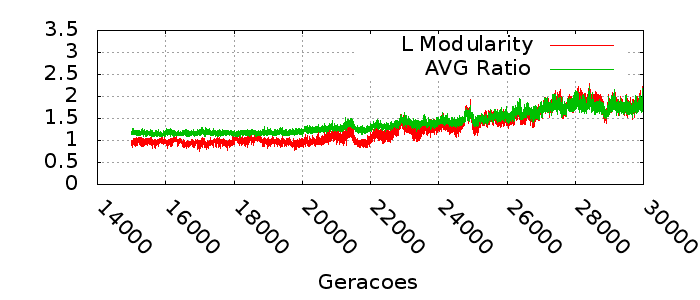
\includegraphics[width=70mm, height=30mm]{figuras/MFMStats70.png}}\vspace{11pt}
      \subfloat [$\Delta_S = 0.08$]{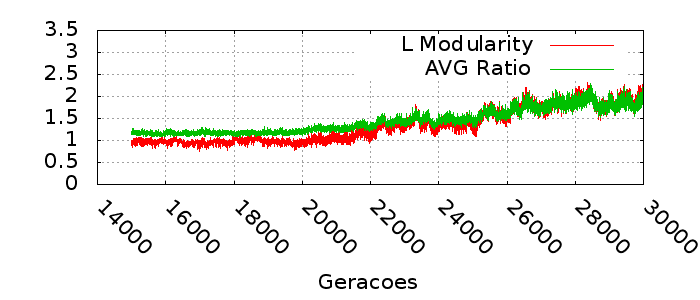
\includegraphics[width=70mm, height=30mm]{figuras/MFMStats80.png}}\\
      \vspace{-18pt}
      \subfloat [$\Delta_S = 0.09$]{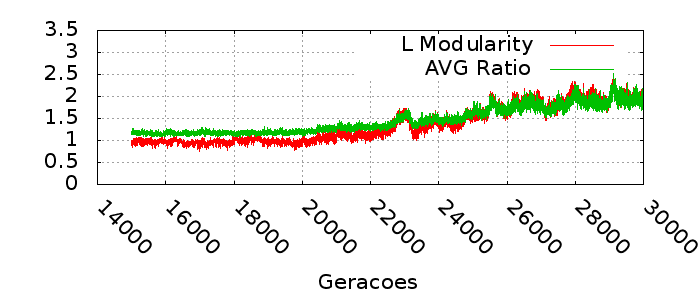
\includegraphics[width=70mm, height=30mm]{figuras/MFMStats90.png}}\vspace{11pt}
      \subfloat [$\Delta_S = 0.1$]{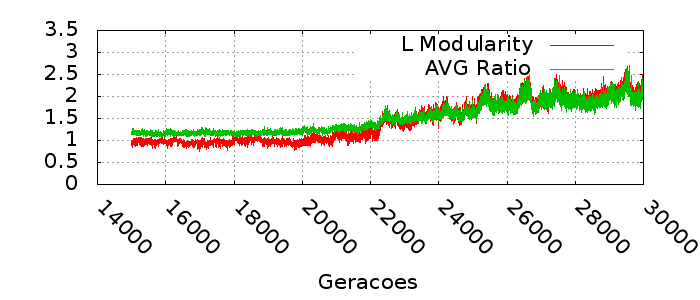
\includegraphics[width=70mm, height=30mm]{figuras/MFMStats100.png}}\\
      \caption{ AVG-Ratio e modularidade $L$ para corridas com
         $\mu/\mu_B = 5$, $Ne = 5000$, $m/p=5$, sofrendo seleção
         estabilizadora correlacionada com 2 módulos e seleção direcional com
         diferentes valores de $\Delta_S$.}
      \label{MFMStats1}
   \end{figure}
\end{center}

\begin{center}
   \begin{figure}[htbp]
      \centering
      \subfloat [$\Delta_S = 0.11$]{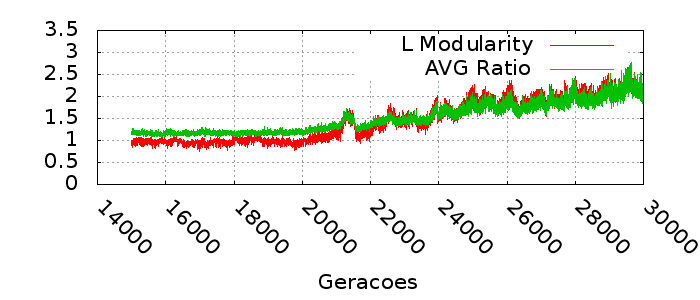
\includegraphics[width=70mm, height=30mm]{figuras/MFMStats110.png}}\vspace{11pt}
      \subfloat [$\Delta_S = 0.12$]{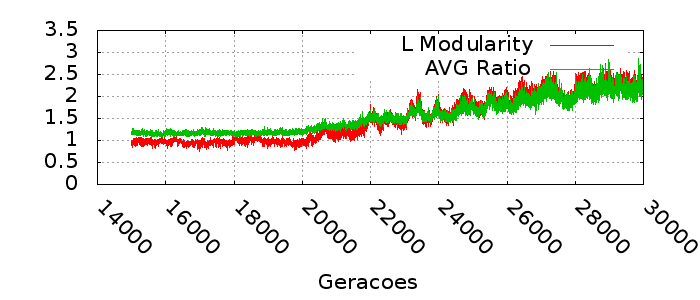
\includegraphics[width=70mm, height=30mm]{figuras/MFMStats120.png}}\\ 
      \vspace{-18pt}
      \subfloat [$\Delta_S = 0.13$]{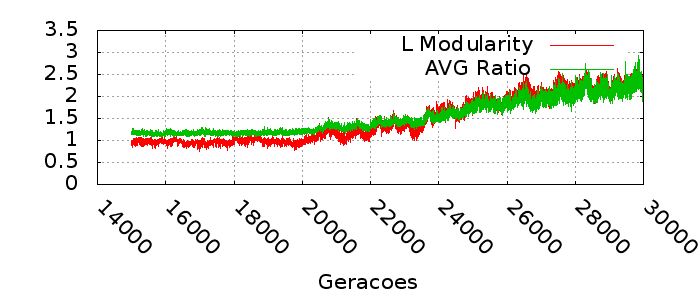
\includegraphics[width=70mm, height=30mm]{figuras/MFMStats130.png}}\vspace{11pt} 
      \subfloat [$\Delta_S = 0.14$]{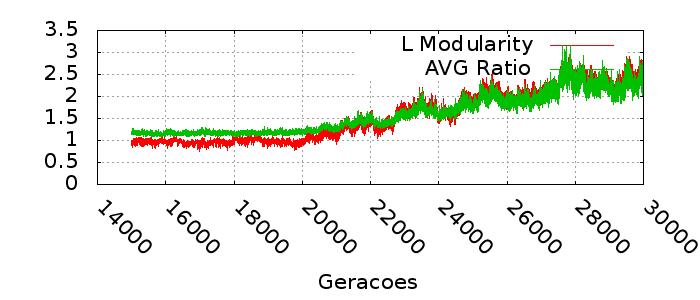
\includegraphics[width=70mm, height=30mm]{figuras/MFMStats140.png}}\\
      \vspace{-18pt}
      \subfloat [$\Delta_S = 0.15$]{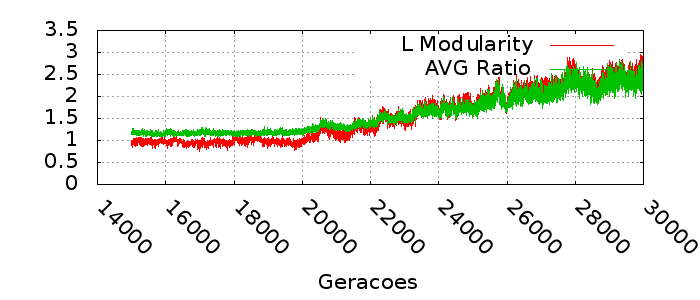
\includegraphics[width=70mm, height=30mm]{figuras/MFMStats150.png}}\vspace{11pt}
      \subfloat [$\Delta_S = 0.16$]{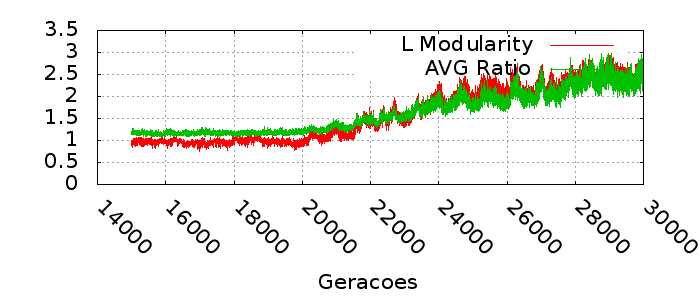
\includegraphics[width=70mm, height=30mm]{figuras/MFMStats160.png}}\\
      \vspace{-18pt}
      \subfloat [$\Delta_S = 0.17$]{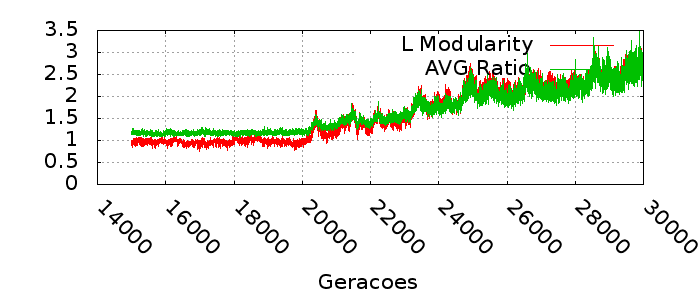
\includegraphics[width=70mm, height=30mm]{figuras/MFMStats170.png}}\vspace{11pt}
      \subfloat [$\Delta_S = 0.18$]{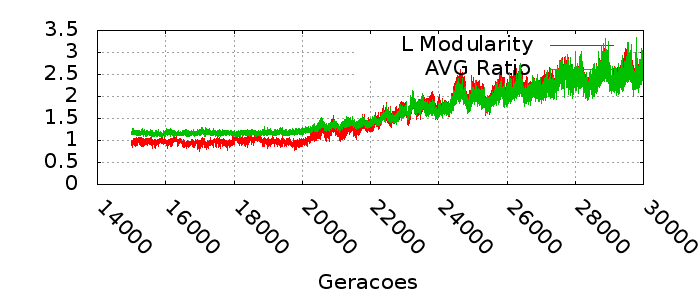
\includegraphics[width=70mm, height=30mm]{figuras/MFMStats180.png}}\\
      \vspace{-18pt}
      \subfloat [$\Delta_S = 0.19$]{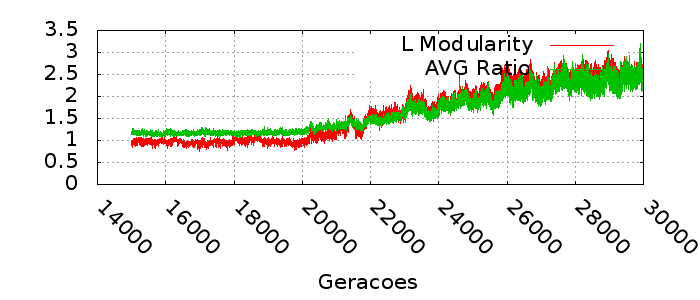
\includegraphics[width=70mm, height=30mm]{figuras/MFMStats190.png}}\vspace{11pt}
      \subfloat [$\Delta_S = 0.2$]{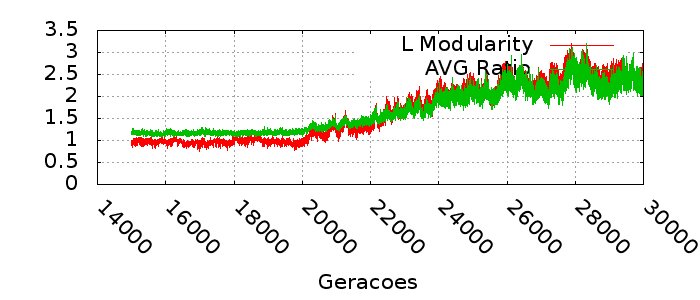
\includegraphics[width=70mm, height=30mm]{figuras/MFMStats200.png}}\\
      \caption{ AVG-Ratio e modularidade $L$ para corridas com
         $\mu/\mu_B = 5$, $Ne = 5000$, $m/p=5$, sofrendo seleção
         estabilizadora correlacionada com 2 módulos e seleção direcional com
         diferentes valores de $\Delta_S$.}
      \label{MFMStats2}
   \end{figure}
\end{center}
